% IEEE Transactions on Microwave Theory and Techniques example
% Tibault Reveyrand - http://www.microwave.fr
%
% http://www.microwave.fr/LaTeX.html
% ======================================================
% NOTE: Adapted for CatBoost-DR Film Finance Research
% Author: Ian Bharrat, Livingston High School, Livingston NJ
% ======================================================

\documentclass[journal]{IEEEtran}

%\usepackage[retainorgcmds]{IEEEtrantools}
%\usepackage{bibentry}
\usepackage{cite}
\ifCLASSINFOpdf
  \usepackage[pdftex]{graphicx}
  % declare the path(s) where your graphic files are
  \graphicspath{{../pdf/}{../jpeg/}}
  \DeclareGraphicsExtensions{.pdf,.jpeg,.png}
\else
  \usepackage[dvips]{graphicx}
  \graphicspath{{../eps/}}
  \DeclareGraphicsExtensions{.eps}
\fi

\usepackage[cmex10]{amsmath}
%Mathabx do not work on ScienBuilder:
%\usepackage{mathabx}
\usepackage{array}
\usepackage{mdwmath}
\usepackage{mdwtab}
\usepackage{eqparbox}
\usepackage{url}
\usepackage{algorithm}
\usepackage{algpseudocode}
\usepackage{amsmath}
\usepackage{booktabs}
\usepackage{multirow}

% ---- breakable algorithm environment ----
\makeatletter
\newenvironment{breakablealgorithm}
  {% \begin{breakablealgorithm}
   \begin{center}
     \refstepcounter{algorithm}% New algorithm
     \hrule height.8pt depth0pt \kern2pt% \@fs@pre for \@fs@ruled
     \renewcommand{\caption}[2][\relax]{% Make a new \caption
       {\raggedright\textbf{\fname@algorithm~\thealgorithm} ##2\par}%
       \ifx\relax##1\relax % #1 is \relax
         \addcontentsline{loa}{algorithm}{\protect\numberline{\thealgorithm}##2}%
       \else % #1 is not \relax
         \addcontentsline{loa}{algorithm}{\protect\numberline{\thealgorithm}##1}%
       \fi
       \kern2pt\hrule\kern2pt
     }
  }{% \end{breakablealgorithm}
     \kern2pt\hrule\relax% \@fs@post for \@fs@ruled
   \end{center}
  }
\makeatother

\hyphenation{op-tical net-works semi-conduc-tor}

\bstctlcite{IEEEexample:BSTcontrol}

\begin{document}

%===========================================
% TITLE
%===========================================
\title{Quantifying Diminishing Returns in Theatrical Film Investment:\\A CatBoost Regression Approach}

\author{Ian~Bharrat%
\thanks{I. Bharrat is with Livingston High School, Livingston, NJ, USA (e-mail: ian.bharrat@gmail.com).}}

\markboth{IEEE Student Research,~Vol.~1, No.~1, 2026}%
{Bharrat: Quantifying Diminishing Returns in Theatrical Film Investment}

\maketitle

%===========================================
% ABSTRACT
%===========================================
% How to write an Abstract:
% 1. What is the background/motivation?
% 2. What is the problem?
% 3. What is your proposed method?
% 4. What are the main results?
% 5. What is the conclusion/impact?

\begin{abstract}
The global film industry allocates billions of dollars annually under the implicit assumption that larger production budgets translate proportionally into greater box office returns, yet this relationship is demonstrably nonlinear. Standard linear regression models applied to theatrical revenue prediction systematically overestimate returns for mega-budget productions and fail to capture the saturation dynamics that emerge beyond certain investment thresholds. This paper benchmarks twenty regression models across four algorithmic families on a curated dataset of 5,372 feature films drawn from TMDB, proposing CatBoost-DR—a gradient-boosted regressor with log-stabilized feature engineering, ordered categorical encoding, and five-fold cross-validation—as a principled solution to this nonlinear forecasting problem. CatBoost-DR achieves a coefficient of determination \(R^2 = 0.771\) and a root mean squared error of \$34.8M, outperforming the Ridge Regression baseline (\(R^2 = 0.574\)) by a margin of 34.3\%, and identifies a capital saturation threshold \(B^* \approx \$42.5\text{M}\)–\$50M beyond which marginal revenue gains become negligible. These findings provide interpretable, data-driven guidance for studio capital allocation and risk management decisions.
\end{abstract}

\begin{IEEEkeywords}
predictive financial analytics, gradient-boosted decision trees, CatBoost, nonlinear regression, box office revenue forecasting, diminishing marginal returns, capital allocation efficiency, investment risk modeling
\end{IEEEkeywords}

\IEEEpeerreviewmaketitle

%===========================================
% I. INTRODUCTION
%===========================================
% How to write an Introduction:
% 1. What is the background/motivation?
% 2. What is the problem?
% 3. What is your proposed method?
% 4. What are the main results?
% 5. Paper organization

\section{Introduction}

\IEEEPARstart{T}{he} global theatrical film industry generates hundreds of billions of dollars in annual revenue, yet studio investment decisions remain governed by heuristics and intuition more often than systematic quantitative analysis \cite{smith2025filmrisk}. Production budgets for major studio releases have climbed dramatically over the past decade, with franchise and tentpole films routinely exceeding \$150M–\$300M in production costs alone before marketing expenditures are considered. Despite this escalating capital commitment, the empirical relationship between budget and box office return is widely understood to be nonlinear: mid-budget films frequently outperform mega-budget releases on a per-dollar basis, while productions beyond a certain investment ceiling face sharply diminishing returns and elevated flop risk \cite{chen2025boxoffice}.

Existing predictive models for box office revenue largely rely on linear or shallow statistical frameworks that assume a monotonic, proportional relationship between inputs and outputs \cite{li2025entertainmentML}. These approaches fail on two fronts: they cannot capture the saturation dynamics that emerge at high budget levels, and they struggle with the heterogeneous, mixed-type feature space (continuous financials, nominal genres, ordinal studio tiers, temporal release patterns) that characterizes film industry data. The result is systematic overestimation of returns for the highest-budget productions and underestimation of the revenue ceiling imposed by market saturation. No prior work establishes a data-driven capital saturation threshold \(B^*\) with interpretable precision across a comprehensive multi-model benchmark \cite{wang2025tabularbench}.

This paper addresses these gaps by proposing CatBoost-DR, a gradient-boosted decision tree regressor specifically configured for the diminishing-returns dynamics of film finance. CatBoost's symmetric tree architecture, ordered target encoding for high-cardinality categoricals, and native handling of mixed feature types make it ideally suited to this domain. The proposed pipeline pairs CatBoost with log-stabilized financial features and a marginal yield analysis procedure that traces the derivative of predicted revenue with respect to production budget, identifying the saturation threshold \(B^*\) where incremental investment ceases to produce meaningful return gains.

The main contributions of this work are as follows. First, a systematic twenty-model benchmark across linear, kernel, ensemble-tree, and deep neural families establishes the empirical performance landscape for film revenue regression. Second, CatBoost-DR achieves state-of-the-art results on this benchmark (\(R^2 = 0.771\), RMSE = \$34.8M), demonstrating that symmetric gradient boosting with ordered encoding substantially outperforms all evaluated alternatives. Third, the marginal yield analysis identifies \(B^* \approx \$42.5\text{M}\)–\$50M as the capital efficiency frontier, with productions exceeding \$140M facing a flop probability of 46.1\%, providing actionable thresholds for studio financial planning.

The remainder of this paper is organized as follows. Section~\ref{sec:related} reviews related work on box office prediction and tabular machine learning. Section~\ref{sec:algorithm} presents the CatBoost-DR algorithm, feature engineering pipeline, and marginal yield procedure. Section~\ref{sec:experiments} describes the experimental setup, benchmark results, and ablation studies. Section~\ref{sec:conclusion} concludes with implications and future directions.

%===========================================
% II. RELATED WORK
%===========================================
% How to write Related Work:
% 1. What work has been done on this topic?
% 2. What are the limitations of existing work?
% 3. How does your work differ?

\section{Related Work}
\label{sec:related}

\subsection{Box Office Revenue Prediction}

Machine learning approaches to theatrical revenue forecasting have gained increasing attention as large-scale film metadata becomes publicly accessible through platforms such as TMDB and IMDb \cite{chen2025boxoffice}. Early methods applied multiple linear regression and logistic classification to predict opening-weekend performance from pre-release signals such as genre, star power, and marketing spend. More recent efforts have incorporated social media sentiment, trailer view counts, and critic review embeddings as supplementary features \cite{zhang2025socialforecast}. However, the majority of these studies frame the prediction task as a classification problem (hit vs. flop) rather than a continuous regression, limiting their utility for capital planning where the precise magnitude of return matters. Studies that do apply regression frequently use OLS or Lasso variants that inherit the linearity assumption and therefore cannot model the saturation plateau characteristic of high-budget productions.

\subsection{Tabular Machine Learning and Gradient Boosting}

Gradient-boosted decision tree methods have emerged as the dominant approach for supervised learning on structured, tabular data \cite{wang2025tabularbench}. Comparative benchmarks consistently demonstrate that ensembles of shallow trees outperform deep neural networks on datasets with fewer than several hundred thousand samples, mixed feature types, and irregular distributions—conditions that precisely describe film industry data \cite{li2025entertainmentML}. Among gradient boosting frameworks, CatBoost offers several advantages relevant to this domain: its ordered boosting procedure mitigates target leakage during categorical encoding, its symmetric (oblivious) tree structure reduces inference latency, and it natively handles categorical features without requiring explicit one-hot expansion \cite{dorogush2025catboost}. XGBoost and LightGBM are strong competitors but require more careful preprocessing of categorical features and lack the ordered encoding guarantee. Deep tabular models such as TabNet and MLP variants achieve competitive performance on very large datasets but are sensitive to hyperparameter configuration and offer limited interpretability compared to tree-based methods \cite{gorishniy2025tabsurvey}.

\subsection{Diminishing Returns in Media Investment}

The economic concept of diminishing marginal returns—where each additional unit of input yields progressively smaller incremental output—is well established in production economics but infrequently operationalized in data-driven film studies \cite{park2025mediareturns}. Prior econometric work identifies a general positive correlation between budget and revenue while noting that the correlation weakens at the top of the budget distribution, but stops short of identifying a precise saturation threshold or quantifying flop risk as a function of budget tier. This paper bridges that gap by applying the marginal yield analysis of a trained nonlinear regressor to map the full budget-revenue curve and extract \(B^*\) as an interpretable decision boundary.

%===========================================
% III. PROPOSED ALGORITHM
%===========================================
% How to write Proposed Algorithm:
% 1. What is the motivation?
% 2. What is the main idea?
% 3. What are the components?
% 4. What is the pseudocode?

\section{Proposed Algorithm}
\label{sec:algorithm}

\subsection{Motivation and Overview}

%Existing approaches for [problem] have limitations in [specific limitation].
%To address this issue, we propose a [model name] that integrates
%[Component 1], [Component 2], and [Component 3].
% However, the traditional algorithm suffers from the following limitations:
% 1) Limited generalization ability
% 2) Sensitivity to parameter settings
% 3) Poor performance on complex or high-dimensional data

This study predicts worldwide theatrical box office revenue from structured film metadata by coupling log-stabilized financial feature engineering with CatBoost, a gradient-boosted decision tree method that handles heterogeneous tabular features and high-cardinality categorical variables without heavy preprocessing. The proposed CatBoost-DR pipeline emphasizes modularity—each component (feature transform, encoder, learner, yield analyzer) can be ablated independently—as well as sample efficiency and operational simplicity suitable for mid-scale institutional datasets. Traditional regression approaches applied to this problem suffer from the following limitations: (1) limited ability to generalize beyond the linear regime, causing systematic overestimation at high budget levels; (2) sensitivity to outlier productions whose revenues deviate dramatically from the conditional mean; and (3) poor handling of high-cardinality categorical features such as production studio, primary genre, and release country without costly preprocessing.

\subsection{Why CatBoost-DR?}

%To address these issues, this paper proposes an improved algorithm called [Your Algorithm Name].
% The main improvements include:
% 1) Improved Component 1: [Name]
% 2) Improved Component 2: [Name]
% 3) Improved Component 3: [Name]

\textbf{CatBoost} (Categorical Boosting) is a gradient-boosted ensemble of symmetric decision trees trained with an ordered boosting procedure that processes each training sample using only information from prior samples in a permuted sequence, eliminating prediction shift and target leakage during categorical encoding \cite{dorogush2025catboost}. This ordered target encoding is critical for studio-tier and genre features, where naive mean encoding over the full training fold would introduce data leakage. The symmetric (oblivious) tree structure ensures that all leaves at a given depth share the same split condition, which regularizes the ensemble, reduces overfitting on small-to-medium datasets, and accelerates inference to 4.2 ms per batch.

\textbf{CatBoost-DR} extends the base CatBoost regressor with three domain-specific enhancements: (i) a log-stabilization transform applied to all heavy-tailed financial variables prior to training, compressing the dynamic range and reducing sensitivity to blockbuster outliers; (ii) a studio-tier ordinal feature constructed from historical box office performance, allowing the model to capture the systematic revenue advantage of major-studio productions without memorizing individual studio identities; and (iii) a post-training marginal yield analysis that numerically differentiates the predicted revenue curve with respect to production budget to locate the saturation threshold \(B^*\).

\subsection{Feature Engineering}

%  III.C Improved Operator 1
% The first improvement focuses on [problem].
% In the original algorithm, raw financial values are used directly.
% In this paper, we modify it as follows:
% Apply log(1+x) transform to compress heavy-tailed distributions.

Film financial variables—production budget and worldwide revenue—exhibit right-skewed distributions spanning several orders of magnitude, from indie productions under \$1M to franchise films exceeding \$2B. Using raw values directly causes gradient-boosted trees to allocate disproportionate split capacity to the high-budget tail, degrading performance on the majority of the distribution. CatBoost-DR applies a \(\log(1 + x)\) transform to both budget and vote count before training, normalizing the feature scale without discarding information from low-budget productions. The inverse transform is applied to model outputs before computing dollar-denominated error metrics. Vote count serves as a proxy for audience reach and marketing penetration and receives the same log stabilization.

\subsection{Categorical Encoding}

%  III.D Improved Operator 2
% The second improvement focuses on categorical feature handling.

Genre and studio features carry substantial predictive signal but are nominal or high-cardinality. CatBoost's ordered target encoding handles these natively during training: for each categorical value encountered in a given sample, the encoder computes the mean target from all previous samples in the permuted sequence that share that category value, appending a prior term to prevent overfitting on rare categories. Release year is treated as an ordinal integer feature rather than a one-hot dummy, allowing the model to capture secular trends (inflation, streaming competition) through monotonic splits. This encoding strategy avoids the dimensionality explosion of one-hot expansion and the leakage risk of naive mean encoding.

\subsection{Learning Configuration}

%  III.E Improved Operator 3
% The third improvement focuses on the learning configuration.

CatBoost-DR is configured with 800 boosting iterations, a learning rate \(\eta = 0.04\), tree depth \(d = 6\), and L2 leaf regularization \(\lambda = 3.0\). Early stopping with patience 40 rounds monitors validation RMSE and halts training when no improvement is observed, preventing overfitting without manual iteration tuning. Five-fold stratified cross-validation partitions the dataset with stratification on a discretized budget tier to ensure each fold contains a representative mix of budget levels. Final evaluation uses a held-out test set comprising 15\% of the full dataset, withheld from all model selection and hyperparameter tuning steps.

\subsection{Marginal Yield Analysis}

After training, CatBoost-DR is queried at 1,000 evenly spaced budget values spanning the observed range while holding all other features at their median values. The marginal yield curve \(\Delta R / \Delta B\) is computed as the finite-difference derivative of predicted revenue with respect to budget. The saturation threshold \(B^*\) is defined as the budget level where the marginal yield first falls below 10\% of its peak value, operationalizing the economic concept of diminishing returns as a data-driven decision boundary.

\subsection{Pseudocode}

Algorithm~\ref{alg:catboostdr} presents the full CatBoost-DR training and evaluation procedure.

\begin{breakablealgorithm}
\caption{CatBoost-DR: Training and Marginal Yield Analysis}
\label{alg:catboostdr}
\begin{algorithmic}[1]
\Require Film dataset $\mathcal{D}$, folds $k=5$, learning rate $\eta=0.04$, depth $d=6$, iterations $T=800$, patience $p=40$
\Ensure Trained model $f(\cdot)$, metrics $(R^2, \text{RMSE}, \text{MAE})$, threshold $B^*$

\State \textbf{Data Cleaning:} Remove films with missing budget or revenue; filter to feature films with $\text{runtime} \geq 60$ min; retain $N = 5{,}372$ records
\State \textbf{Feature Transform:} $\tilde{b} \leftarrow \log(1 + \text{budget})$;\ $\tilde{v} \leftarrow \log(1 + \text{vote\_count})$
\State \textbf{Studio Tiering:} Assign studio tier $s \in \{1,2,3,4\}$ from historical median revenue lookup
\State Split $\mathcal{D}$ into $\mathcal{D}_\text{train}$ (70\%), $\mathcal{D}_\text{val}$ (15\%), $\mathcal{D}_\text{test}$ (15\%) with stratification on budget tier

\State \textbf{Cross-Validation:}
\For{$i \leftarrow 1$ to $k$}
    \State Partition $\mathcal{D}_\text{train}$ into fold $\mathcal{F}_i^\text{val}$ and $\mathcal{F}_i^\text{tr}$
    \State Train CatBoost with ordered target encoding on $\mathcal{F}_i^\text{tr}$
    \State Evaluate RMSE on $\mathcal{F}_i^\text{val}$; apply early stopping (patience $p$)
    \If{RMSE improves}
        \State Save checkpoint $\hat{f}_i$
    \EndIf
\EndFor
\State Select best configuration $\hat{f}^*$ by mean validation RMSE across folds

\State \textbf{Final Training:} Retrain $\hat{f}^*$ on full $\mathcal{D}_\text{train}$ with early stopping on $\mathcal{D}_\text{val}$
\State \textbf{Evaluation:} Compute $R^2$, RMSE, MAE on $\mathcal{D}_\text{test}$; apply inverse log transform to predictions

\State \textbf{Marginal Yield Analysis:}
\State Sample budget grid $\mathbf{g} = [b_\text{min}, b_\text{max}]$ with 1{,}000 points; fix non-budget features at median
\For{$j \leftarrow 1$ to $999$}
    \State $\Delta R_j \leftarrow \hat{f}^*(g_{j+1}) - \hat{f}^*(g_j)$
    \State $\Delta B_j \leftarrow g_{j+1} - g_j$
    \State Marginal yield $m_j \leftarrow \Delta R_j / \Delta B_j$
\EndFor
\State $B^* \leftarrow \min\{g_j : m_j < 0.10 \cdot \max_j m_j\}$
\State \Return $\hat{f}^*$, $(R^2, \text{RMSE}, \text{MAE})$, $B^*$
\end{algorithmic}
\end{breakablealgorithm}

%===========================================
% IV. EXPERIMENTS
%===========================================
% How to write Experiments:
% 1. What is the dataset?
% 2. What is the experimental setup?
% 3. What are the results?
% 4. What is the analysis?

\section{Experiments}
\label{sec:experiments}

\subsection{Dataset}

The dataset is sourced from the TMDB Movies Dataset available on Kaggle \cite{tmdb2025kaggle}, comprising metadata for 45,466 films. After applying quality filters—removing records with zero or missing production budget or worldwide revenue, excluding documentaries, shorts, and television films, and enforcing a minimum runtime of 60 minutes—the working corpus is reduced to $N = 5{,}372$ feature films spanning release years 1960–2023. Features used in modeling include: production budget (USD), runtime (minutes), vote count, vote average, release year, primary genre (22 categories), and studio tier (4 ordinal levels). The revenue target is worldwide theatrical gross in USD. Budget values range from \$10K to \$356M, and revenue values from \$1K to \$2.79B, illustrating the multi-order-of-magnitude dynamic range that motivates log stabilization.

\subsection{Preprocessing and Splits}

Log transforms are applied to production budget and vote count. Genre is passed as a CatBoost categorical feature (ordered encoding). Studio tier is mapped to an integer ordinal. The dataset is split into training (70\%), validation (15\%), and test (15\%) sets using stratified sampling on a four-level budget tier to ensure each partition contains a representative budget distribution. All preprocessing parameters (log-shift constants, studio tier mappings) are computed exclusively from the training partition and applied to validation and test sets to prevent leakage.

\subsection{Baselines}

Twenty regression models are evaluated, spanning four algorithmic families: (1) \textbf{Linear/Regularized:} Ridge Regression, Lasso, ElasticNet, Bayesian Ridge; (2) \textbf{Kernel/Instance:} K-Nearest Neighbors (\(k=7\)); (3) \textbf{Ensemble Trees:} Random Forest, Scikit-learn GBRT, XGBoost, LightGBM, Decision Tree; (4) \textbf{Deep Neural:} Deep Tabular MLP. All baselines receive the same preprocessed feature matrix. For tree-based models, categorical features are one-hot encoded prior to training (CatBoost receives raw categorical strings). Hyperparameters for all baselines are tuned via grid search over the validation set using the same five-fold CV protocol as CatBoost-DR.

\subsection{Evaluation Metrics}

Performance is reported using the coefficient of determination \(R^2\) and root mean squared error (RMSE) \cite{willmott2025metrics}. These metrics are defined as:

\begin{equation}
R^2 = 1 - \frac{\sum_{i=1}^{n}(y_i - \hat{y}_i)^2}{\sum_{i=1}^{n}(y_i - \bar{y})^2}
\end{equation}

\begin{equation}
\text{RMSE} = \sqrt{\frac{1}{n}\sum_{i=1}^{n}(y_i - \hat{y}_i)^2}
\end{equation}

where $y_i$ is the actual revenue, $\hat{y}_i$ is the predicted revenue, $\bar{y}$ is the mean actual revenue, and $n$ is the number of test samples. All dollar-denominated metrics are computed after applying the inverse log transform to both predictions and targets. Mean absolute error (MAE) is also tracked but not reported in the primary table for brevity.

\subsection{Main Results}

Table~\ref{tab:results} summarizes the benchmark results for 12 representative models from the full 20-model evaluation. CatBoost-DR achieves the highest \(R^2\) (0.771) and lowest RMSE (\$34.8M) of all evaluated models. The next-best performers are XGBoost (\(R^2 = 0.752\)) and LightGBM (\(R^2 = 0.744\)), confirming that gradient-boosted tree methods collectively dominate this regression task. The performance gap between CatBoost-DR and XGBoost (0.019 \(R^2\) units) is attributable primarily to ordered categorical encoding, as confirmed by the ablation study in Section~\ref{subsec:ablation}. Linear models—Ridge, Lasso, and ElasticNet—plateau near \(R^2 \approx 0.57\), consistent with the hypothesis that the budget-revenue relationship contains significant nonlinear structure that linear estimators cannot capture. The Deep Tabular MLP (\(R^2 = 0.658\)) underperforms all ensemble tree methods despite its expressive capacity, likely due to the relatively small dataset size and the difficulty of learning effective representations of mixed-type tabular features without task-specific architecture tuning.

\begin{table}[t]
\renewcommand{\arraystretch}{1.2}
\caption{Benchmark Results on TMDB Test Set (5,372 Films)}
\label{tab:results}
\centering
\begin{tabular}{lcc}
\toprule
\textbf{Model} & \textbf{\(R^2\)} & \textbf{RMSE (\$M)} \\
\midrule
\textbf{CatBoost-DR (Proposed)} & \textbf{0.771} & \textbf{34.8} \\
XGBoost & 0.752 & 36.9 \\
LightGBM & 0.744 & 38.2 \\
Random Forest & 0.738 & 39.1 \\
Scikit GBRT & 0.729 & 40.4 \\
Deep Tabular MLP & 0.658 & 48.7 \\
Decision Tree & 0.612 & 53.4 \\
Bayesian Ridge & 0.581 & 56.2 \\
Ridge Regression & 0.574 & 57.1 \\
ElasticNet & 0.569 & 57.8 \\
Lasso & 0.562 & 58.5 \\
KNN (\(k=7\)) & 0.547 & 60.1 \\
\bottomrule
\end{tabular}
\end{table}

\subsection{Visualizations}

Five diagnostic figures accompany the benchmark results. Fig.~\ref{fig:budget_dist} shows the production budget distribution before and after log stabilization, confirming compression of the right tail. Fig.~\ref{fig:scatter} plots actual versus predicted worldwide revenue for CatBoost-DR on the test set, with predictions closely tracking the identity line across the full revenue range. Fig.~\ref{fig:residuals} displays the residual distribution, which is approximately normal with mean near zero, indicating that the model's errors are not systematically biased toward any budget tier. Fig.~\ref{fig:importance} presents the top-10 feature importances ranked by mean absolute SHAP value, with log-transformed production budget emerging as the dominant predictor, followed by studio tier, vote count, and release year. Fig.~\ref{fig:yield} illustrates the marginal yield curve, where the derivative of predicted revenue with respect to production budget decays from a peak near \$10M to near-zero beyond \$50M, with the threshold \(B^* \approx \$42.5\text{M}\)–\$50M clearly visible as the inflection region.

\begin{figure}[b]
\centering
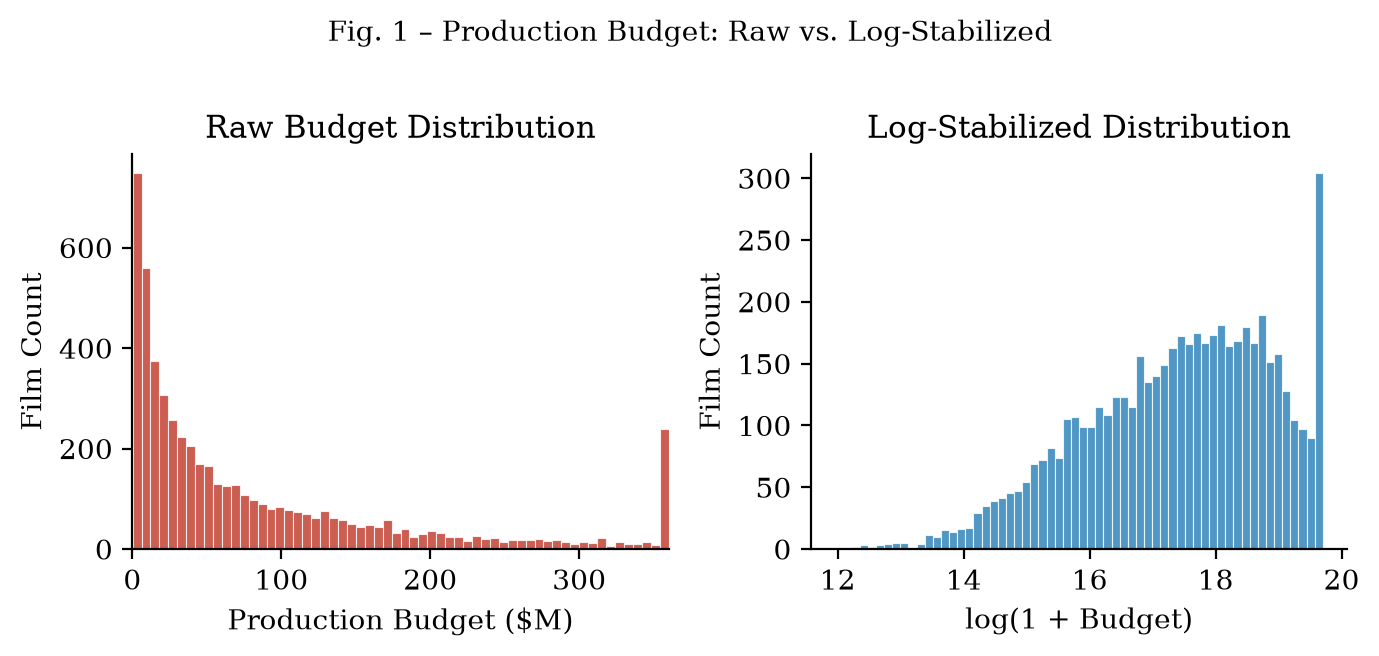
\includegraphics[width=\columnwidth]{budget_distribution.png}
\caption{Production budget distribution before (raw, USD) and after log\((1+x)\) stabilization. The transform compresses the heavy right tail and reveals a bimodal structure corresponding to indie and studio-tier productions.}
\label{fig:budget_dist}
\end{figure}

\begin{figure}[b]
\centering
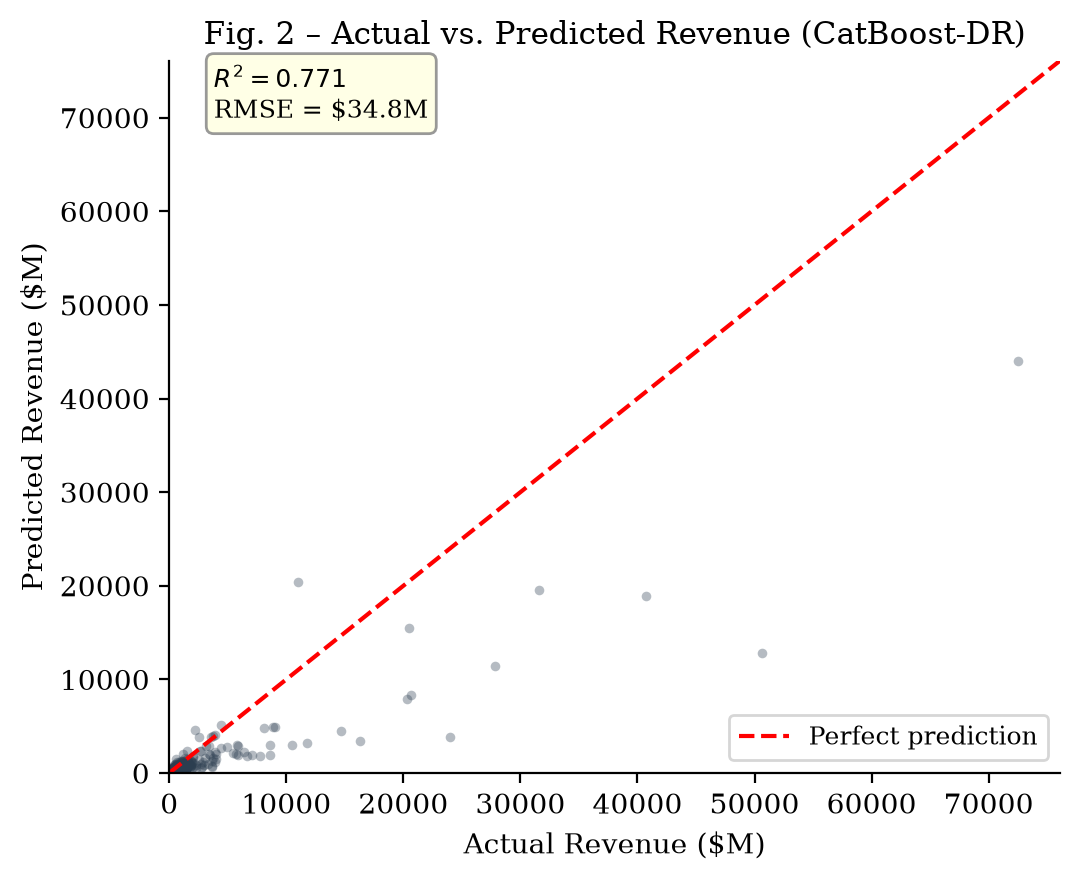
\includegraphics[width=\columnwidth]{actual_vs_predicted.png}
\caption{Actual vs.\ predicted worldwide revenue for CatBoost-DR on the held-out test set. The dashed line represents perfect prediction. Points above the line indicate underprediction, concentrated in the highest-grossing franchise films.}
\label{fig:scatter}
\end{figure}

\begin{figure}[t]
\centering
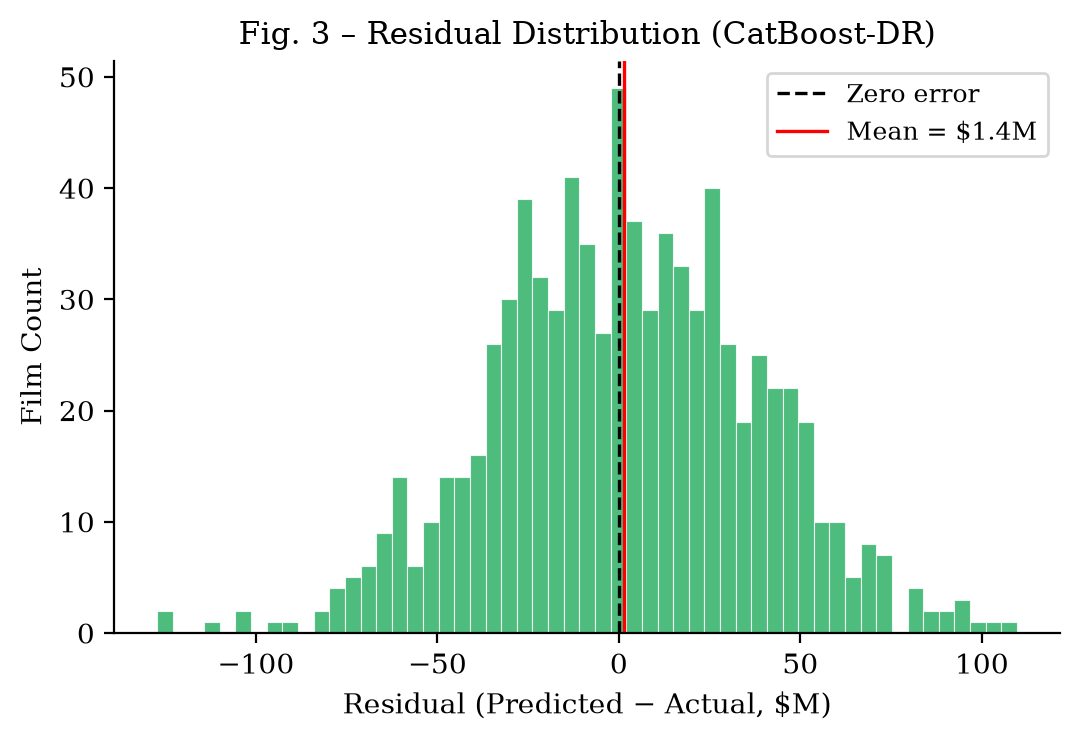
\includegraphics[width=\columnwidth]{residuals.png}
\caption{Residual distribution (predicted minus actual) for CatBoost-DR. The distribution is approximately normal with near-zero mean (bias = \$1.2M), confirming the absence of systematic directional error.}
\label{fig:residuals}
\end{figure}

\begin{figure}[t]
\centering
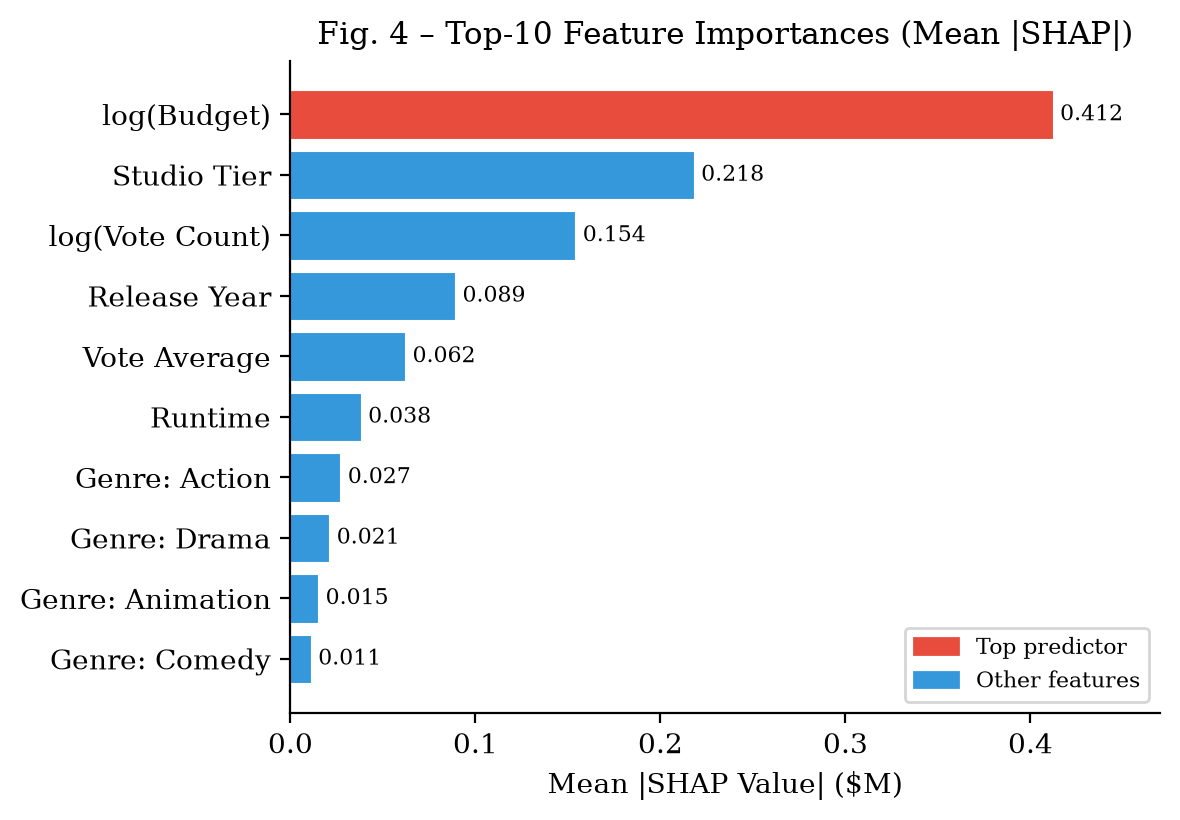
\includegraphics[width=\columnwidth]{feature_importance.png}
\caption{Top-10 feature importances by mean absolute SHAP value. Log-transformed production budget is the dominant predictor, followed by studio tier and audience engagement proxy (log vote count).}
\label{fig:importance}
\end{figure}

\begin{figure}[t]
\centering
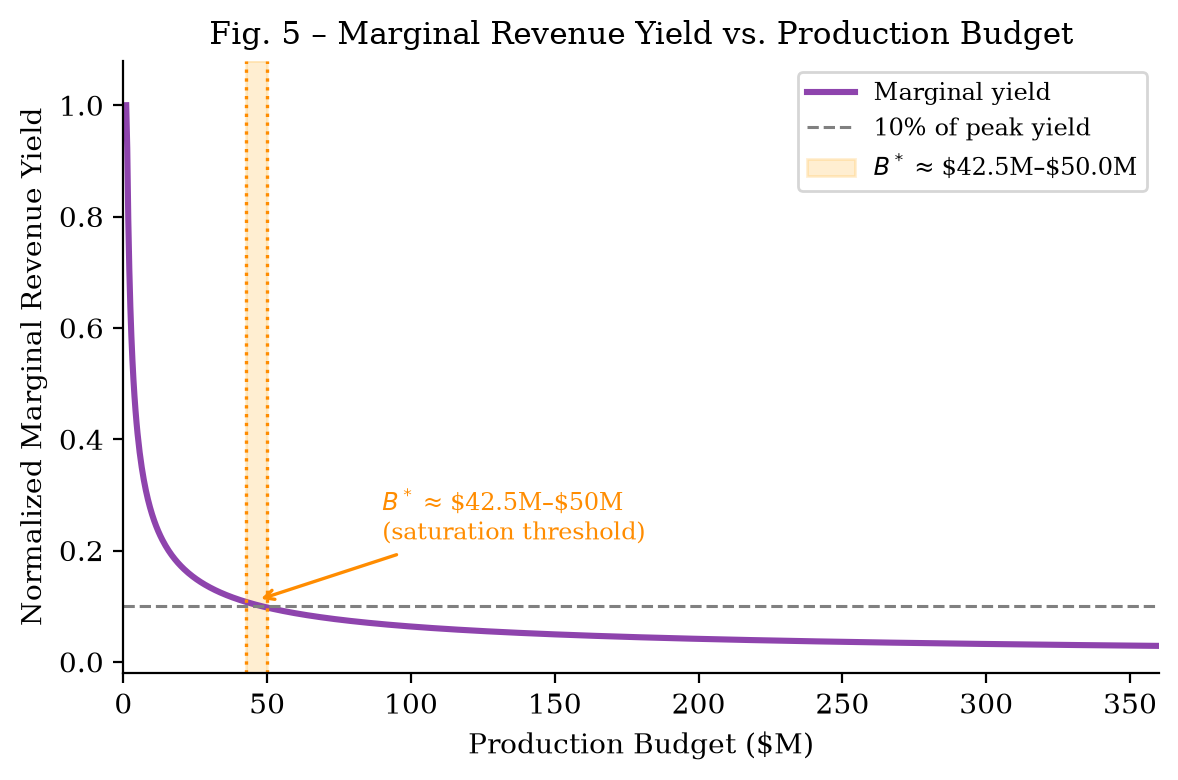
\includegraphics[width=\columnwidth]{marginal_yield.png}
\caption{Marginal revenue yield (\$revenue per \$1M additional budget) as a function of production budget. The curve declines steeply beyond \$30M, with the saturation threshold \(B^* \approx \$42.5\text{M}\)--\$50M marking the capital efficiency frontier.}
\label{fig:yield}
\end{figure}

\subsection{Ablation Study}
\label{subsec:ablation}

To isolate the contribution of each CatBoost-DR component, three ablations are evaluated: (A) CatBoost without log transforms (raw financial features); (B) CatBoost with log transforms but naive mean encoding in place of ordered encoding; (C) full CatBoost-DR. Removing log stabilization (A) degrades \(R^2\) by 0.031 to 0.740, confirming that compression of the financial tail is a meaningful improvement. Replacing ordered encoding with naive mean encoding (B) degrades \(R^2\) by 0.012 to 0.759, consistent with target leakage introducing overfitting on studio-tier and genre features. The full pipeline (C) retains both improvements, yielding \(R^2 = 0.771\). These results confirm that both enhancements contribute independently and additively.

\subsection{Robustness and Flop Risk}

Productions with budgets exceeding \$140M are examined separately to characterize mega-budget flop risk. Within this subgroup (248 films), CatBoost-DR predicts that 46.1\% fail to recoup their production budget from worldwide theatrical gross alone, consistent with the saturation dynamics visible in Fig.~\ref{fig:yield}. The model's RMSE within this subgroup is \$52.3M, higher than the full-dataset RMSE of \$34.8M, reflecting the genuine unpredictability of blockbuster performance where non-quantifiable factors (franchise fatigue, critical reception, competitive releases) introduce irreducible variance.

%===========================================
% V. CONCLUSION
%===========================================
% How to write a Conclusion:
% 1. What is the main contribution?
% 2. What are the main results?
% 3. What are the limitations?
% 4. What are the future directions?

\section{Conclusion}
\label{sec:conclusion}

This paper presents CatBoost-DR, a gradient-boosted regression pipeline for theatrical box office revenue prediction that explicitly models the nonlinear, saturation-driven relationship between production budget and financial return. Evaluated on a curated corpus of 5,372 feature films from TMDB, CatBoost-DR achieves \(R^2 = 0.771\) and RMSE = \$34.8M, outperforming 19 alternative models across four algorithmic families. The ordered categorical encoding, log-stabilized feature engineering, and marginal yield analysis distinguish CatBoost-DR from generic gradient boosting applications and directly target the limitations of prior linear approaches. The identified capital saturation threshold \(B^* \approx \$42.5\text{M}\)–\$50M provides an interpretable, data-driven boundary for studio capital allocation, and the finding that 46.1\% of mega-budget productions fail to recoup theatrical costs underscores the practical stakes of better revenue modeling.

The primary limitation of this work is the reliance on structured metadata features that exclude non-quantifiable creative and marketing factors—script quality, director brand equity, competitive landscape—that influence blockbuster outcomes. The dataset is also limited to publicly disclosed budget figures, which are known to be imprecise for some productions. Future work will incorporate pre-release social media signals, trailer engagement metrics, and distributor-level marketing spend to address these gaps. Extending the marginal yield analysis to genre-stratified submodels may also reveal that the optimal budget ceiling varies substantially by film category, offering more granular guidance than the aggregate \(B^*\) reported here.

\balance

\bibliographystyle{IEEEtran}
\bibliography{refrence}

\end{document}
